\chapter{Supervised Learning} % (fold)
\label{cha:supervised_learning}

\marginnote{From CS229 Fall 2020, Tengyu Ma, Andrew Ng \& Chris R\'e, Stanford University.}

\section{Linear Predictors} % (fold)
\label{sec:linear_predictors}

We now embark on our journey into machine learning with the simplest yet most practical tool: \textit{linear predictors}, which cover both \textit{classification} and \textit{regression} and are examples of \textit{reflex models}.
% 
After getting some geometric intuition for linear predictors, we will turn to learning the \textit{weights} of a linear predictor by formulating an optimization problem based on the \textit{loss minimization} framework.
% 
Finally, we will discuss \textit{stochastic gradient descent}, an efficient algorithm for optimizing (that is, minimizing) the loss that's tailored for machine learning which is much faster than \textit{gradient descent}.

\begin{example}
    \bparagraph{Example application: spam classification.}
    
    \br

    \textbf{Input:} $x = \text{email message}$

    \textbf{Output:} $y = \{ \text{spam}, \text{not-spam}\}$

    \textbf{Objective:} obtain a \textit{predictor} $f$:
    \[
        x \longrightarrow \boxed{f} \longrightarrow y
    \]
\end{example}
First, some terminology. A \textit{predictor} is a function $f$ that maps an \textit{input} $x$ to an \textit{output} $y$. In statistics, $y$ is known as a response, and when $x$ is a real vector, it is known as the \textit{covariate}.

% section linear_predictors (end)



\subsection{Types of Prediction Tasks} % (fold)
\label{sub:types_of_prediction_tasks}

In the context of classification tasks, $f$ is called a \textit{classifier} and $y$ is called a \textit{label} (sometimes \textit{class}, \textit{category}, or \textit{tag}). The key distinction between binary classification and regression is that the former has discrete outputs (e.g., "yes" or "no"), whereas the latter has continuous outputs.
Note that the dichotomy of prediction tasks are not meant to be formal definitions, but rather to provide intuition.
For instance, binary classification could technically be seen as a regression problem if the labels are $-1$ and $+1$. And structured prediction generally refers to tasks where the possible set of outputs $y$ is huge (generally, exponential in the size of the input), but where each individual $y$ has some structure. For example, in machine translation, the output is a sequence of words.

\begin{itemize}
    \item \textbf{Binary classification:} (e.g., email $\implies$ spam/not spam)
    \[
        x \longrightarrow \boxed{f} \longrightarrow y \in \{+1, -1\}
    \]

    \item \textbf{Regression:} (e.g., location, year $\implies$ housing price)
    \[
        x \longrightarrow \boxed{f} \longrightarrow y \in \mathbb{R}
    \]

    \item \textbf{Multiclass classification:} $y$ is a category
    \[
        \text{picture} \longrightarrow \boxed{f} \longrightarrow \text{``cat''}
    \]

    \item \textbf{Ranking:} $y$ is a permutation % TODO?
    \[
        \boxed{1}~\boxed{2}~\boxed{3}~\boxed{4} \longrightarrow \boxed{f} \longrightarrow 2~3~4~1
    \]

    \item \textbf{Structured prediction:} $y$ is an object which is built from parts
    \[
        \textit{``la casa blu''} \longrightarrow \boxed{f} \longrightarrow \textit{``the blue house''}
    \]
\end{itemize}

% subsection types_of_prediction_tasks (end)

% \pagebreak

\subsection{Data} % (fold)
\label{sub:data}

The starting point of machine learning is the \textit{data}.
For now, we will focus on \textit{supervised learning}, in which our data provides both inputs and outputs, in contrast to unsupervised learning, which only provides inputs.
A (supervised) \textit{example} (also called a \textit{data point} or \textit{instance}) is simply an input-output pair $(x,y)$, which specifies that $y$ is the ground-truth output for $x$.
The \textit{training data} $\Dtrain$ is a multiset of examples (repeats are allowed, but this is not important), which forms a partial specification of the desired behavior of a predictor.

\begin{example} 
    \bparagraph{Data example:} specifies that $y$ is the ground-truth output for $x$
    \[
        (x,y)
    \]

    \bparagraph{Training data:} list of examples for spam classification
    \[
        \Dtrain = \begin{bmatrix}
            (``\ldots10\text{m dollars}\ldots'',+1) \\
            (``\ldots \text{CS}221\ldots'',-1)
        \end{bmatrix}
    \]
    \[
        \textit{partial specification of behavior}
    \]
\end{example}

% subsection data (end)


\subsection{Learning} % (fold)
\label{sub:learning}

% TODO: tikz
\marginnote{
\begin{gather*}
    % \textbf{\underline{framework}}\\
    \Dtrain \longrightarrow \boxed{\textbf{learner}} \longrightarrow \begin{matrix}x \\ \downarrow \\ \boxed{f} \\ \downarrow \\ y\end{matrix}
    % (x \to f \to y)
\end{gather*}
}

\textit{Learning} is about taking the training data $\Dtrain$ and producing a predictor $f$, which is a function that takes inputs $x$ and tries to map them to outputs $y=f(x)$. One thing to keep in mind is that we want the predictor to approximately work even for examples that we have not seen in $\Dtrain$. This problem of generalization, which we will discuss two chapters from now, forces us to design $f$ in a principled, mathematical way.
We will first focus on examining what $f$ is, independent of how the learning works. Then we will come back to learning $f$ based on data.

% subsection learning (end)

% \pagebreak

\subsection{Feature Extraction} % (fold)
\label{sub:feature_extraction}

We will consider predictors $f$ based on \textit{feature extractors} $\phi$. Feature extraction is a bit of an art that requires intuition about both the task and also what machine learning algorithms are capable of.

The general principle is that features should represent properties of $x$ which might be relevant for predicting $y$. It is okay to add features which turn out to be irrelevant, since the learning algorithm can sort it out (though it might require more data to do so).

\begin{example}

\bparagraph{Example: feature extractor.}

\br

\textbf{Example task}: predict $y$, indicating whether a string $x$ is an email address.

\textbf{Question:} what properties of $x$ might be relevant for predicting $y$?

\textbf{Feature extractor:}\\
\indent\indent Given input $x$, output a set of (feature name, feature value) pairs.
\[
\texttt{"abc@gmail.com"} \xrightarrow[\text{arbitrary!}]{\text{feature extractor}} \begin{bmatrix}
\texttt{length>10}: & 1\\
\texttt{fracOfAlpha}: & 0.85\\
\texttt{contains\_@}: & 1\\
\texttt{endsWith\_.com}: & 1\\
\texttt{endsWith\_.org}: & 0
\end{bmatrix}
\]
% TODO: colors (red "feature name", blue "feature value")

\begin{exalgorithm}
\begin{juliaverbatim}
# Indicator function \bbI
𝕀(b) = b ? 1 : 0

# Feature extrator \phi
φ = x -> [𝕀(length(x) > 10),
         sum(isletter(xᵢ) for xᵢ in x)/length(x),
         𝕀(occursin("@", x)),
         𝕀(endswith(x, ".com")),
         𝕀(endswith(x, ".org"))]
\end{juliaverbatim}
\end{exalgorithm}

\jlconglobal{../jl/support_code.jl}
\begin{juliaconsole}
x = "abc@gmail.com";
φ(x)
\end{juliaconsole}

\caption{
    \label{ex:feature_extrator}
    A \textit{feature extractor} for classifying whether a string is an email address.
    The indicator function symbol \jlv{𝕀} can be created by typing \jlv{\bbI} and hitting tab and the feature extractor symbol \jlv{φ} symbol with \jlv{\phi}.
}
\end{example}

\paragraph{Feature Vector Notation}

Each input $x$ represented by a \textit{feature vector} $\phi(x)$, which is computed by the feature extractor $\phi$.
When designing features, it is useful to think of the feature vector as being a map from strings (feature names) to doubles (feature values).
But formally, the feature vector $\phi(x) \in \mathbb{R}^d$ is a real vector $\phi(x) = [\phi_1(x), \dots, \phi_d(x)]$, where each component $\phi_j(x)$, for $j = 1, \dots, d$, represents a feature.

\begin{example}% TODO: \definition env.
\bparagraph{Definition: feature vector.} For an input $x$, its feature vector is:
\[
    \phi(x) = [\phi_1(x), \dots, \phi_d(x)]
\]
Think of $\phi(x) \in \mathbb{R}^d$ as a point in a high-dimensional space.
\end{example}

This vector-based representation allows us to think about feature vectors as a point in a (high-dimensional) vector space, which will later be useful for getting some geometric intuition.
% 
Mathematically, feature vector doesn't need feature names:
\[
\phi(x) = \begin{bmatrix} % TODO: Fix colon alignment
\texttt{length>10}: & 1\\
\texttt{fracOfAlpha}: & 0.85\\
\texttt{contains\_@}: & 1\\
\texttt{endsWith\_.com}: & 1\\
\texttt{endsWith\_.org}: & 0
\end{bmatrix} = \begin{bmatrix}
1\\
0.85\\
1\\
1\\
0
\end{bmatrix}
\]


% subsection feature_extraction (end)

\subsection{Weight Vector} % (fold)
\label{sub:weight_vector}

% \paragraph{Weight Vector} % (fold)
\label{par:weight_vector}
So far, we have defined a feature extractor $\phi$ that maps each input $x$ to the feature vector $\phi(x)$.
A \textit{weight vector} $\vec{w} = [w_1, \dots, w_d]$ (also called a \textit{parameter vector} or \textit{weights})
specifies the contributions of each feature vector to the prediction.
% For each feature $j$, we have a real number $w_j$ representing contribution of feature to prediction.
\[
\vec{w} = \begin{bmatrix}
\texttt{length>10}: & -1.2\\
\texttt{fracOfAlpha}: & 0.6\\
\texttt{contains\_@}: & 3\\
\texttt{endsWith\_.com}: & 2.2\\
\texttt{endsWith\_.org}: & 1.4
\end{bmatrix} = \begin{bmatrix}
-1.2\\
0.6\\
3\\
2.2\\
1.4
\end{bmatrix}
\]

In the context of binary classification with binary features
$(\phi_j(x) \in \{0,1\})$, the weights $w_j \in \R$ have an intuitive interpretation.
If $w_j$ is positive, then the presence of feature $j$ $(\phi_j(x) = 1)$ favors a positive classification.
Conversely, if $w_j$ is negative, then the presence of feature $j$ favors a negative classification.

Note that while the feature vector depends on the input $x$, the weight vector does not.
This is because we want a single predictor (specified by the weight vector) that works on any input.


% paragraph weight_vector (end)

% subsection weight_vector (end)

\begin{example}
    \bparagraph{Definition: score.}

    The score on an example $(x,y)$ is $\vec{w}\cdot \phi(x)$, how \textit{confident} we are in predicting $+1$. Score is a weighted combination of features:
    \[
        \vec{w} \cdot \phi(x) = \sum_{j=1}^d w_j \phi(x)_j
    \]
\end{example}

\begin{algorithm}
\begin{juliaverbatim}
score(x, 𝐰, φ) = 𝐰⋅φ(x)
\end{juliaverbatim}

\caption{
    \label{alg:score}
    The \textit{score} of input \jlv{x} using weights \jlv{𝐰} and feature extractor \jlv{φ} written in the Julia programming language.
    The \jlv{dot} product symbol \jlv{⋅} can be created by typing \jlv{\cdot} and hitting tab (included in the \jlv{LinearAlgebra} package), and the \jlv{𝐰} symbol with \jlv{\bfw}.
}
\end{algorithm}

Given a feature vector $\phi(x)$ and a weight vector $\vec{w}$, we define the prediction \textit{score} to be their inner product.
The score intuitively represents the degree to which the classification is positive or negative.
The predictor is linear because the score is a linear function of $\vec{w}$ (more on linearity in the next chapter).
Again, in the context of binary classification with binary features, the score aggregates the contribution of each feature, weighted appropriately.
We can think of each feature present as voting on the classification.


\begin{example}
    % TODO: add code, expand.
    \bparagraph{Example: score.}
    \[\begin{aligned}
        \text{weight vector: }\, \vec{w} \in \R^d & \qquad & \text{feature vector: }\, \phi(x) \in \R^d\\
        \begin{bmatrix}
            \texttt{length>10}: & -1.2\\
            \texttt{fracOfAlpha}: & 0.6\\
            \texttt{contains\_@}: & 3\\
            \texttt{endsWith\_.com}: & 2.2\\
            \texttt{endsWith\_.org}: & 1.4
        \end{bmatrix} & \qquad & \begin{bmatrix}
            \texttt{length>10}: & 1\\
            \texttt{fracOfAlpha}: & 0.85\\
            \texttt{contains\_@}: & 1\\
            \texttt{endsWith\_.com}: & 1\\
            \texttt{endsWith\_.org}: & 0
        \end{bmatrix}
    \end{aligned}\]
    \[\vec{w}\cdot\phi(x) = -1.2(1) + 0.6(0.85) + 3(1) + 2.2(1) + 1.4(0) = 4.51\]
\begin{juliaconsole}
x = "abc@gmail.com";
𝐰 = [-1.2, 0.6, 3, 2.2, 1.4];
score(x, 𝐰, φ)
\end{juliaconsole}
% 𝐰⋅φ(x)

\caption{
    \label{ex:score}
    Calculating \textit{score} as the weighted sum of features with feature extractor \jlv{φ} from \cref{ex:feature_extrator}.
}
\end{example}




\subsection{Binary Classification} % (fold)
\label{sub:binary_classification}

We now have gathered enough intuition that we can formally define the predictor $f$.
For each weight vector $\vec{w}$, we write $f_{\vec{w}}$ to denote the predictor that depends on $\vec{w}$
and takes the sign of the score.
For this section, we will focus on the case of \textit{binary classification}. % DIFF: "slides" to "section"
For weight vector $\vec{w} \in \R^d$ and feature vector $\phi(x) \in \R^d$, a (binary) linear classifier is defined as:
\[
    f_{\vec{w}}(x) = \sign(\vec{w} \cdot \phi(x)) = \begin{cases}
        +1 & \text{if }\vec{w} \cdot \phi(x) > 0\\
        -1 & \text{if }\vec{w} \cdot \phi(x) < 0\\
        \text{?} & \text{if }\vec{w} \cdot \phi(x) = 0
    \end{cases}
\]
Recall that in this setting, we call the predictor a (binary) classifier.
The case of $f_{\vec{w}}(x) =~?$ is a boundary case that isn't so important.
We can just predict $+1$ arbitrarily as a matter of convention.
\[
    f_{\vec{w}}(x) = \sign(\vec{w} \cdot \phi(x)) = \begin{cases}
        +1 & \text{if }\vec{w} \cdot \phi(x) \ge 0\\
        -1 & \text{otherwise}
    \end{cases}
\]
% -1 & \text{if }\vec{w} \cdot \phi(x) < 0
\begin{algorithm}
\begin{juliaverbatim}
binary_classifier(x, 𝐰, φ) = score(x, 𝐰, φ) ≥ 0 ? +1 : -1
\end{juliaverbatim}

\caption{
    \label{alg:binary_classifier}
    A \textit{binary classifier} $f$ to classify input \jlv{x} using weight vector \jlv{𝐰} and feature extractor \jlv{φ}. We predict $+1$ when the score is zero as a matter of convention.
}
\end{algorithm}

% subsection binary_classification (end)

\subsection{Geometric Intuition} % (fold)
\label{sub:geometric_intuition}
So far, we have talked about linear predictors as weighted combinations of features.
We can get a bit more insight by studying the \textit{geometry} of the problem.
Let's visualize the predictor $f_{\vec{w}}$ by looking at which points it classifies positive.
Specifically, we can draw a ray from the origin to $\vec{w}$ (in two dimensions).
Points which form an acute angle with $\vec{w}$ are classified as positive (dot product is positive),
and points that form an obtuse angle with $\vec{w}$ are classified as negative.
Points which are orthogonal $\{ z \in \R^d : \vec{w} \cdot z = 0 \}$ constitute the \textit{decision boundary}.
By changing $\vec{w}$, we change the predictor $f_{\vec{w}}$ and thus the decision boundary as well.

\begin{example}
    Example:
    \begin{gather*}     
        \vec{w} = [2,-1]\\
        \phi(x) \in \{[2,0],[0,2],[2,4]\}
    \end{gather*}
    In general: binary classifier $f_{\vec{w}}$ defines a hyperplane \textbf{decision boundary} with normal vector $\vec{w}$.
    % TODO: Whiteboard example

    $\mathbb{R}^2$: hyperplane is a line

    $\mathbb{R}^3$: hyperplane is a plane
\end{example}

% subsection geometric_intuition (end)



\section{Loss Minimization} % (fold)
\label{sec:loss_minimization}
So far we have talked about linear predictors $f_{\vec{w}}$ which are based on a feature extractor $\phi$ and a weight vector $\vec{w}$.
Now we turn to the problem of estimating (also known as \textit{fitting} or \textit{learning}) $\vec{w}$ from training data.
The \textit{loss minimization} framework is to cast learning as an optimization problem.
Note the theme of separating your problem into a model (optimization problem) and an algorithm (optimization algorithm).

% \marginnote{
\begin{gather*}
    % \textbf{\underline{framework}}\\
    \Dtrain \longrightarrow \boxed{\textbf{learner}} \longrightarrow \begin{matrix}x \\ \downarrow \\ \boxed{f} \\ \downarrow \\ y\end{matrix}
\end{gather*}
% }
\begin{gather*}
    \boxed{\textbf{learner}} = \boxed{\boxed{\text{\textcolor{green!50!black}{optimization problem}}} \longrightarrow \boxed{\text{\textcolor{orange!50!black}{optimization algorithm}}}}
\end{gather*}

\begin{example}
    \bparagraph{Definition: loss function.} A loss function $\operatorname{Loss}(x,y,\vec{w})$ quantifies how unhappy you would be if you used $\vec{w}$ to make a prediction on $x$ when the correct output is $y$. It is the object we want to minimize.
\end{example}

% section loss_minimization (end)

\subsection{Score and Margin} % (fold)
\label{sub:score_and_margin}
% \textbf{Correct label:} $y$

% \textbf{Predicted label:} $y^\prime = f_{\vec{w}}(x) = \sign(\vec{w} \cdot \phi(x))$

% \textbf{Example:} $\vec{w} = [2, -1], \phi(x) = [2, 0], y = -1$

Recal that the \textit{score} on an example $(x,y)$ is $\vec{w}\cdot \phi(x)$ which is how \textit{confident} we are in predicting $+1$.
Before we talk about what loss functions look like and how to learn $\vec{w}$,
we introduce another important concept, the notion of a \textit{margin}.
Suppose the correct label is $y \in \{-1,+1\}$.
The margin of an input $x$ is $\vec{w} \cdot \phi(x) y$, which measures how correct the prediction that $\vec{w}$ makes is.
The larger the margin the better, and non-positive margins correspond to classification errors.

\begin{example}
    \bparagraph{Definition: margin.} The margin on an example $(x,y)$ is how \textit{correct} we are:
    \[
        (\vec{w}\cdot\phi(x))y = \text{score} \times \text{target}
    \]
\end{example}

\begin{algorithm}
\begin{juliaverbatim}
margin(x, y, 𝐰, φ) = score(x, 𝐰, φ)*y
\end{juliaverbatim}

\caption{
    \label{alg:margin}
    The \textit{margin} of an example \jlv{(x,y)} using weights \jlv{𝐰} and feature extractor \jlv{φ}.
}
\end{algorithm}
Note that if we look at the actual prediction $f_{\vec{w}}(x)$,
we can only ascertain whether the prediction was right or not.
By looking at the score and the margin, we can get a more nuanced view into the behavior of the classifier.

Geometrically, if $\|\vec{w}\| = 1$, then the margin of an input $x$ is exactly the distance from its feature vector $\phi(x)$ to the \textit{decision boundary}.

\begin{example}
    \bparagraph{Question:} When does a binary classifier err on an example?
    \begin{itemize}
        \item margin less than $0$ % Answer.
        \item margin greater than $0$
        \item score less than $0$
        \item score greater than $0$
    \end{itemize}
    % TODO: Julia code for hints (also to fill in space here to remove \pagebreak)
\end{example}

% subsection score_and_margin (end)

\pagebreak


% \begin{example}
%   \textbf{Example:} $\vec{w} = [2, -1], \phi(x) = [2, 0], y = -1$

%   \br

%   \textbf{Recall the binary classifier:}
%   \[
%   f_{\vec{w}}(x) = \sign(\vec{w} \cdot \phi(x))
%   \]
%   % TODO: Whiteboard? 
% \end{example}

% \bparagraph{Definition: zero-one loss.} 

Now let us define our first loss function, the \textit{zero-one loss}.
This corresponds exactly to our familiar notion of whether our predictor made a mistake or not.
We can also write the loss in terms of the margin.
\begin{marginfigure}
    \caption{
        \label{fig:zero_one_loss} \textit{Zero-one loss}.
    }
  \begin{jlcode}
  p = let
      ymin = 0
      ymax = 4

      plots = Plots.Plot[
          Plots.Linear(
              x->Loss_01(x, +1, [1], x->x), (-3,3), xbins=1000, style="solid, ultra thick, mark=none, red", legendentry=L"\ZeroOneLoss"
          ),
      ]
      Axis(plots,
           xlabel=L"\text{margin}~(\mathbf{w}\cdot\phi(x))y",
           ylabel=L"\ZeroOneLoss(x,y,\mathbf{w})",
           style="ymajorgrids, enlarge x limits=0, ymin=$ymin, ymax=$ymax, legend pos=north west, legend style={at={(0.5,-0.5)},anchor=north}",
           width="5cm", height="4cm")
  end
  plot(p)
  \end{jlcode}
  \begin{center}
    \plot{fig/zero_one_loss}
  \end{center}
\end{marginfigure}
\begin{align*}
\ZeroOneLoss(x, y, \vec{w}) &= \mathbb{1}[f_{\vec{w}}(x) \neq y]\\
                            &= \mathbb{1}[\underbrace{(\vec{w} \cdot \phi(x)) y}_\text{margin} \le 0]
\end{align*}

% TODO: graph.
%   parentCenter('$\\red{\\ZeroOneLoss}(x, y, \\w) = \\mathbb{1}[(\\w \\cdot \\phi(x)) y \\le 0]$
We can plot the loss as a function of the margin.
From the graph, it is clear that the loss is $1$ when the margin is negative and $0$ when it is positive.

\begin{algorithm}
\begin{juliaverbatim}
Loss_01_f(x, y, 𝐰, φ, f) = 𝕀(f(x, 𝐰, φ) ≠ y)
Loss_01(x, y, 𝐰, φ) = 𝕀(margin(x, y, 𝐰, φ) ≤ 0)
\end{juliaverbatim}

\caption{
    \label{alg:zero_one_loss}
    The \textit{zero-one loss} function for an example \jlv{(x,y)} using weights \jlv{𝐰}, feature extractor \jlv{φ}, and classifier \jlv{f}. Note that \jlv{Loss_01} performs binary classification using the \jlv{margin}.
}
\end{algorithm}

\subsection{Linear Regression} % (fold)
\label{sub:linear_regression}

% TODO: Graph.

Now let's turn for a moment to regression, where the output $y$ is a real number rather than $\{-1,+1\}$.
Here, the \textit{zero-one loss} doesn't make sense, because it's unlikely that we're going to predict $y$ exactly.

\begin{marginfigure}[10mm]
  \begin{jlcode}
    p = let
        ymin = 0
        ymax = 3

        plots = Plots.Plot[
            Plots.Linear(
                x->x*3/4, (0,4), style="solid, ultra thick, mark=none, red"
            ),
            Plots.Scatter(2, 2.5, mark="*", markSize=1, style="mark options={fill=darkgreen}, darkgreen"),
            Plots.Linear([2, 2], [2.5, 1.5], mark="none", style="dashed, black"),
            Plots.Node("\\shortstack{\\footnotesize residual\\\\\$\\mathbf{w}\\cdot\\phi(x) - y\$}", 1.1, 2),
            Plots.Node("\\footnotesize \$(\\phi(x), y)\$", 2.55, 2.5),
        ]
        Axis(plots,
             title=L"f_{\mathbf{w}}(x) = \mathbf{w}\cdot\phi(x)",
             xlabel=L"\phi(x)",
             ylabel=L"\mathbf{w}\cdot\phi(x)",
             style="ymajorgrids, enlarge x limits=0, ymin=$ymin, ymax=$ymax, legend pos=north west, legend style={at={(0.5,-0.5)},anchor=north}",
             width="6cm", height="4cm")
    end
    plot(p)
  \end{jlcode}
  \begin{center}
    \plot{fig/residual}
  \end{center}

\caption{
\label{fig:residual} \textit{Residual}.
}
\end{marginfigure}
Let's instead define the \textit{residual} to measure how close the prediction $f_{\vec{w}}(x)$ is to the correct $y$.
The residual will play the analogous role of the margin for classification and will let us craft an appropriate loss function.
\begin{example}
    \bparagraph{Definition: residual.} The \textit{residual} is the amount by which the prediction $f_{\vec{w}}(x)=\vec{w} \cdot \phi(x)$ overshoots the target $y$:
    \[
        (\vec{w} \cdot \phi(x)) - y = \text{score} - \text{target}
    \]
\end{example}

\begin{algorithm}
\begin{juliaverbatim}
residual(x, y, 𝐰, φ) = score(x, 𝐰, φ) - y
\end{juliaverbatim}

\caption{
    \label{alg:residual}
    The \textit{residual} of an example \jlv{(x,y)} using weights \jlv{𝐰}, and feature extractor \jlv{φ}.
}
\end{algorithm}
% \begin{example}
%   \bparagraph{Definition: squared loss.} 
% \end{example}
% Example was here.

% \pagebreak

% subsection linear_regression (end)

\subsection{Regression Loss Functions} % (fold)
\label{sec:regression_loss_functions}

A popular and convenient loss function to use in linear regression is the \textit{squared loss},
which penalizes the residual of the prediction quadratically.
If the predictor is off by a residual of $10$, then the loss will be $100$.
\begin{marginfigure}[-5mm]
    % \caption{
    %     \label{fig:squared_loss} \textit{Squared loss} and \textit{absolute deviation loss}.
    % }
  \begin{jlcode}
    p = let
        ymin = 0
        ymax = 4

        plots = Plots.Plot[
            Plots.Linear(
                x->0.5*Loss_squared(x, 0, [1], x->x), (-3,3), style="solid, ultra thick, mark=none, stanfordred", legendentry=L"\SquaredLoss"
            ),
        ]
        Axis(plots,
             xlabel=L"\text{residual}~(\mathbf{w}\cdot\phi(x)) - y",
             ylabel=L"\Loss(x,y,\mathbf{w})",
             style="ymajorgrids, enlarge x limits=0, ymin=$ymin, ymax=$ymax, legend pos=north west, legend style={at={(0.5,-0.5)},anchor=north}",
             width="5cm", height="4cm")
    end
    plot(p)
  \end{jlcode}
  \begin{center}
    \plot{fig/squared_loss}
  \end{center}
\end{marginfigure}
\begin{equation*}
\begin{aligned}
    \SquaredLoss(x, y, \vec{w}) &= (f_{\vec{w}}(x) - y)^2\\
                                &= (\underbrace{\vec{w} \cdot \phi(x)-y}_\text{residual})^2
\end{aligned}
\end{equation*}
\begin{algorithm}
\begin{juliaverbatim}
Loss_squared(x, y, 𝐰, φ) = residual(x, y, 𝐰, φ)^2
\end{juliaverbatim}
% Loss_squared(x, y, 𝐰, φ, f) = (f(x, 𝐰, φ) - y)^2

\caption[][-5mm]{
    \label{alg:squared_loss}
    The \textit{squared loss} for an example \jlv{(x,y)} using weights \jlv{𝐰}, and feature extractor \jlv{φ}.
    % Note that \jlv{Loss_squared_residual} ...
}
\end{algorithm}

An alternative to the squared loss is the \textit{absolute deviation loss},
which simply takes the absolute value of the residual.
\begin{marginfigure}[5mm]
    % \caption{
    %     \label{fig:squared_loss_absdev_loss} \textit{Squared loss} and \textit{absolute deviation loss}.
    % }
  \begin{jlcode}
    p = let
        ymin = 0
        ymax = 4

        plots = Plots.Plot[
            Plots.Linear(
                x->0.5*Loss_squared(x, 0, [1], x->x), (-3,3), style="solid, ultra thick, mark=none, stanfordred", legendentry=L"\SquaredLoss"
            ),
            Plots.Linear(
                x->Loss_absdev(x, 0, [1], x->x), (-3,3), style="solid, ultra thick, mark=none, darkgreen", legendentry=L"\AbsDevLoss"
            ),
        ]
        Axis(plots,
             xlabel=L"\text{residual}~(\mathbf{w}\cdot\phi(x)) - y",
             ylabel=L"\Loss(x,y,\mathbf{w})",
             style="ymajorgrids, enlarge x limits=0, ymin=$ymin, ymax=$ymax, legend pos=north west, legend style={at={(0.5,-0.5)},anchor=north}",
             width="5cm", height="4cm")
    end
    plot(p)
  \end{jlcode}
  \begin{center}
    \plot{fig/squared_loss_absdev_loss}
  \end{center}
\end{marginfigure}
\begin{equation*}
\begin{aligned}
    \AbsDevLoss(x, y, \vec{w}) &= |f_{\vec{w}}(x) - y|\\
                                &= |\underbrace{\vec{w} \cdot \phi(x)-y}_\text{residual}|
\end{aligned}
\end{equation*}
\begin{algorithm}
\begin{juliaverbatim}
Loss_absdev(x, y, 𝐰, φ) = abs(residual(x, y, 𝐰, φ))
\end{juliaverbatim}

\caption[][8mm]{
    \label{alg:abs_dev_loss}
    The \textit{absolute deviation loss} for an example \jlv{(x,y)} using weights \jlv{𝐰}, and feature extractor \jlv{φ}.
}
\end{algorithm}
\begin{overflowexample}
    \bparagraph{Example of $\SquaredLoss$ and $\AbsDevLoss$:}
    \begin{gather*}
        \vec{w} = [2, -1], \phi(x) = [2, 0], y = -1\\
        \SquaredLoss(x, y, \vec{w}) = 25\\
        \AbsDevLoss(x, y, \vec{w}) = 5
    \end{gather*}
\begin{juliaconsole}
𝐰 = [2, -1]; φ = x->[2, 0]; y = -1; x = missing
Loss_squared(x, y, 𝐰, φ)
Loss_absdev(x, y, 𝐰, φ)
\end{juliaconsole}
\end{overflowexample}

% subsection regression_loss_functions (end)

\subsection{Loss Minimization Framework} % (fold)
\label{sub:loss_minimization_framework}

So far: one example, $\Loss(x, y, \vec{w})$ is easy to minimize.
% 
Note that on one example, both the squared and absolute deviation loss functions have the same minimum,
so we cannot really appreciate the differences here.
However, we are learning $\vec{w}$ based on a whole training set $\Dtrain$,
not just one example.
We typically minimize the \textit{training loss} (also known as the training error or empirical risk), which is the average loss over all the training examples.
\begin{example} % TODO: red
\textbf{Key idea: minimize training loss}
\begin{gather*}
    \TrainLoss(\vec{w}) = \frac{1}{|\Dtrain|} \sum_{(x,y) \in \Dtrain} \operatorname{Loss}(x,y,\vec{w})\\
    \minimize_{\vec{w} \in \mathbb{R}^d} \TrainLoss(\vec{w})
\end{gather*}
Key: need to set $\vec{w}$ to make global tradeoffs---not every example can be happy.
\end{example}
\begin{algorithm}
\begin{juliaverbatim}
function TrainLoss(𝐰, 𝒟train, φ, Loss)
    return sum(Loss(x,y,𝐰,φ) for (x,y) ∈ 𝒟train)/length(𝒟train)
end

minimize(𝒟train, φ, Loss) =
    minimize(𝐰->TrainLoss(𝐰, 𝒟train, φ, Loss))
\end{juliaverbatim}

\caption{
    \label{alg:trainloss} \textit{Training loss} for weights \jlv{𝐰} and data \jlv{𝒟train} using feature extractor \jlv{φ} and loss function \jlv{Loss}.
}
\end{algorithm}

Importantly, such an optimization problem requires making tradeoffs across all the examples
(in general, we won't be able to set $\vec{w}$ to a single value that makes every example have low loss).

% subsection loss_minimization_framework (end)

\begin{example}
    \bparagraph{Which regression loss to use?}
    % = \{ (1, 0), (1, 2), (1, 1000) \}$
    For the training data $\Dtrain$ and feature vector $\phi(x) = x$, the weight $\vec{w}$ that minimizes the \textit{least squares} ($L_2$) regression training loss is the \textbf{mean} $y$. The mean tries to accommodate every example, i.e. popular.
    % \blue{
    \[
      \operatorname{Loss}_\text{squared}(x, y, \vec{w}) = (\vec{w} \cdot \phi(x) - y)^2
    \]
    For \textit{least absolute deviation} ($L_1$) regression, the weights $\vec{w}$ that minimizes the training loss is the \textbf{median} $y$. The median is more robust to outliers.
    \[
      \operatorname{Loss}_\text{absdev}(x, y, \vec{w}) = |\vec{w} \cdot \phi(x) - y|
    \]
\end{example}

Now the question of which loss we should use becomes more interesting.
For example, consider the case where all the inputs are $\phi(x) = 1$.
Essentially the problem becomes one of predicting a single value $y^*$ which is the least offensive towards all the examples.

If our loss function is the squared loss, then the optimal value is the mean $y^* = \frac{1}{|\Dtrain|} \sum_{(x,y) \in \Dtrain} y$.
If our loss function is the absolute deviation loss, then the optimal value is the median.
The median is more robust to outliers: you can move the furthest point arbitrarily farther out without affecting the median.
This makes sense given that the squared loss penalizes large residuals a lot more.

In summary, this is an example of where the choice of the loss function has a qualitative impact on the weights learned,
and we can study these differences in terms of the objective function without thinking about optimization algorithms.

\begin{marginfigure}
  \begin{jlcode}
    p = let
        ymin = 0
        ymax = 8
        𝒟train = [(1,1)] # x ∈ ℝ

        φ = x->x
        bias = 1

        x_opt = gradient_descent(𝒟train, φ, ∇TrainLoss)
        y_opt = TrainLoss(x_opt, 𝒟train, φ, Loss_squared)+bias

        plots = Plots.Plot[
            Plots.Linear(
                𝐰->TrainLoss(𝐰, 𝒟train, φ, Loss_squared)+bias, (-3,3), style="solid, ultra thick, mark=none, stanfordred"
            ),
            Plots.Scatter(x_opt, y_opt, mark="*", markSize=1.5, style="mark options={fill=black}, white")
        ]
        Axis(plots,
             title=L"\mathbf{w} \in \mathbb{R}",
             xlabel=L"\text{weight}~\mathbf{w}",
             ylabel=L"\TrainLoss(\mathbf{w})",
             style="ymajorgrids, enlarge x limits=0, ymin=$ymin, ymax=$ymax, legend pos=north west, legend style={at={(0.5,-0.5)},anchor=north}",
             width="5cm", height="4cm")
    end
    plot(p)
  \end{jlcode}
  \begin{center}
    \plot{fig/trainloss}
  \end{center}
    \caption{
        \label{fig:trainloss} \textit{Training loss} in $\mathbb{R}$ with minimum.
    }
\end{marginfigure}
\begin{marginfigure}
  \begin{jlcode}
    using ColorSchemes
    pasteljet = ColorMaps.RGBArrayMap(ColorSchemes.viridis, interpolation_levels=500, invert=true)
    p = let
        w = 20
        𝒟train = [([3,0.7],4), ([-1,0.3],3), ([-1,-3],0)] # x ∈ ℝ²
        φ = x->x

        plots = Plots.Plot[
            Plots.Image((𝐰1,𝐰2)->TrainLoss([𝐰1,𝐰2], 𝒟train, φ, Loss_squared), (-w,w), (-w,w), colormap=pasteljet, colorbar=false),
            Plots.Scatter(gradient_descent(𝒟train, φ, ∇TrainLoss)..., mark="*", markSize=1, style="mark options={fill=white}, black")
        ]
        Axis(plots,
             title=L"\mathbf{w} \in \mathbb{R}^2",
             xlabel=L"w_1",
             ylabel=L"w_2",
             style="enlarge x limits=0, xticklabels={,,}, yticklabels={,,},",
             width="5cm", height="4cm")
    end
    plot(p)
  \end{jlcode}
  \begin{center}
    \plot{fig/trainloss2d}
  \end{center}
    \caption{
        \label{fig:trainloss2d} \textit{Training loss} in $\mathbb{R}^2$ with minimum.
    }
\end{marginfigure}

\section{Optimization Problem} % (fold)
\label{sec:optimization_problem}
% TODO: Plots.
Having defined a bunch of different objective functions that correspond to training loss, 
we would now like to optimize them---that is, obtain an algorithm that outputs the $\vec{w}$ where the objective function achieves the minimum value.
% \text{objective:} 
\[
    \minimize_{\vec{w} \in \mathbb{R}^d} \TrainLoss(\vec{w})
\]

\subsection{Gradient Descent} % (fold)
\label{sub:gradient_descent}


\begin{example}
    \bparagraph{Definition: gradient.} The gradient $\nabla_{\vec{w}}\TrainLoss(\vec{w})$ is the direction that increases the loss the most.
\end{example}

\begin{algorithm}[ht]
\caption{\label{alg:gd}Gradient descent.}
\begin{algorithmic}
  \Function{GradientDescent}{$\Train, \nabla\TrainLoss$}  
    \State Initialize $\vec{w}=[0,\ldots,0]$
    \For{$t = 1,\ldots,T$}:
        \State $\vec{w} \leftarrow \vec{w} - \underbrace{\eta}_{\text{step size}} \underbrace{\nabla_{\vec{w}}\TrainLoss(\vec{w})}_{\text{gradient}}$
    \EndFor
\EndFunction
\end{algorithmic}
\end{algorithm}
\begin{algorithm}
\begin{juliaverbatim}
init_weights(d) = d == 1 ? zero(d) : zeros(d)

function gradient_descent(𝒟train, φ, ∇TrainLoss; η=0.1, T=100)
    𝐰 = init_weights(length(φ(𝒟train[1][1])))
    for t in 1:T
        𝐰 = 𝐰 - η*∇TrainLoss(𝐰, 𝒟train, φ)
    end
    return 𝐰
end
\end{juliaverbatim}

\caption{
    \label{alg:gradient_descent}
    \textit{Gradient descent} on the weights \jlv{𝐰} to minimize the \textit{least squares} training loss function over the training data \jlv{𝒟train} using feature extractor \jlv{φ}, step size \jlv{η}, and number of iterations \jlv{T}.
}
\end{algorithm}
A general approach is to use \textit{iterative optimization}, which essentially starts at some starting point $\vec{w}$ (say, all zeros),
and tries to tweak $\vec{w}$ so that the objective function value decreases.

To do this, we will rely on the gradient of the function, which tells us which direction to move in to decrease the objective the most.
The gradient is a valuable piece of information, especially since we will often be optimizing in high dimensions ($d$ on the order of thousands).

This iterative optimization procedure is called \textit{gradient descent}.
Gradient descent has two \textit{hyperparameters}, the \textit{step size} $\eta$ (which specifies how aggressively we want to pursue a direction) and the number of iterations $T$.
Let's not worry about how to set them, but you can think of $T = 100$ and $\eta = 0.1$ for now.

% subsection gradient_descent (end)

% section optimization_problem (end)

\subsection{Least Squares Regression} % (fold)
\label{sub:least_squares_regression}

All that's left to do before we can use gradient descent is to compute the gradient of our objective function $\TrainLoss$.
The calculus can usually be done by hand; combinations of the product and chain rule suffice in most cases for the functions we care about.
% 
Note that the gradient often has a nice interpretation.
For squared loss, it is the residual ($\text{prediction} - \text{target}$) times the feature vector $\phi(x)$.
Our objective function is:
\[
  \displaystyle \TrainLoss(\vec{w}) = \frac{1}{|\Dtrain|} \sum_{(x,y) \in \Dtrain} (\vec{w} \cdot \phi(x) - y)^2
\]
Compute the gradient using the chain rule:
\begin{align*}
\displaystyle \nabla_{\vec{w}} \TrainLoss(\vec{w}) &= \frac{1}{|\Dtrain|} \sum_{(x,y) \in \Dtrain} \nabla_{\vec{w}}\SquaredLoss(x, y, \vec{w})\\
                                                   &= \frac{1}{|\Dtrain|} \sum_{(x,y) \in \Dtrain} 2 (\underbrace{\vec{w} \cdot \phi(x) - y}_{\substack{\text{prediction} - \text{target} \\ \text{(residual)}}}) \phi(x)
\end{align*}

Note that for linear predictors, the gradient is always something times $\phi(x)$ because $\vec{w}$ only affects the loss through $\vec{w} \cdot \phi(x)$.
\begin{algorithm}
\begin{juliaverbatim}
∇Loss_squared(x, y, 𝐰, φ) = 2residual(x, y, 𝐰, φ)*φ(x)

function ∇TrainLoss(𝐰, 𝒟train, φ)
    return sum(∇Loss_squared(x, y, 𝐰, φ)
        for (x,y) ∈ 𝒟train)/length(𝒟train)
end
\end{juliaverbatim}

\caption{
    \label{alg:gradient_trainloss}
    \textit{Training loss gradient} for \textit{least squares regression}.
}
\end{algorithm}

% subsection least_squares_regression (end)

\subsection{Gradient Descent is Slow} % (fold)
\label{sub:gradient_descent_is_slow}
The problem with gradient descent is each iteration requires going over all training examples---which is expensive when you have lots of data!
\[
  \w \leftarrow \w - \eta \nabla_{\w} \TrainLoss(\w)
\]

We can now apply gradient descent on any of our objective functions that we defined before and have a working algorithm.
But it is not necessarily the best algorithm.
% 
One problem (but not the only problem) with gradient descent is that it is slow.
Those of you familiar with optimization will recognize that methods like Newton's method can give faster convergence,
but that's not the type of slowness I'm talking about here.
% 
Rather, it is the slowness that arises in large-scale machine learning applications.
Recall that the training loss is a sum over the training data.
If we have one million training examples (which is, by today's standards, only a modest number),
then each gradient computation requires going through those one million examples, and this must happen before we can make any progress.
Can we make progress before seeing all the data?

% subsection gradient_descent_is_slow (end)

% \pagebreak % TODO: remove?

\subsection{Stochastic Gradient Descent} % (fold)
\label{sub:stochastic_gradient_descent}
% Stochastic gradient descent (SGD):

In \textit{stochastic gradient descent} (SGD), % DIFF: "The answer is..."
rather than looping through all the training examples to compute a single gradient and making one step,
SGD loops through the examples $(x,y)$ and updates the weights $\w$ based on \textit{each} example.
Each update is not as good because we're only looking at one example rather than all the examples, but we can make many more updates this way.
% \[
%     \displaystyle \TrainLoss(\w) = \frac{1}{|\Dtrain|} \sum_{(x,y) \in \Dtrain} \Loss(x, y, \w)
% \]

\begin{algorithm}[ht]
  \caption{Stochastic gradient descent.}
  % \label{alg:gd}
  \begin{algorithmic}
  \Function{StochasticGradientDescent}{$\Train, \nabla\Loss$}  
    \State Initialize $\vec{w}=[0,\ldots,0]$
    \For{$t = 1,\ldots,T$}:
        \For{$(x,y) \in \Dtrain$}:
            \State $\w \leftarrow \w - \eta \nabla_{\w} \Loss(x, y, \w)$
        \EndFor
    \EndFor
  \EndFunction
  \end{algorithmic}
  \bparagraph{Key idea: stochastic updates.} It's not about \textit{quality}, it's about \textit{quantity}.
\end{algorithm}
\begin{algorithm}
\begin{juliaverbatim}
function stochastic_gradient_descent(𝒟train, φ, ∇Loss; η=0.1)
    𝐰 = init_weights(length(φ(𝒟train[1][1])))
    for t in 1:T
        for (x,y) ∈ 𝒟train
            𝐰 = 𝐰 - η*∇Loss(x, y, 𝐰, φ)
        end
    end
    return 𝐰
end
\end{juliaverbatim}

\caption{
    \label{alg:sgd}
    \textit{Stochastic gradient descent} over training data \jlv{𝒟train} using feature extractor \jlv{φ} and gradient of the loss function \jlv{∇Loss} and step size \jlv{η}.
}
\end{algorithm}


In practice, we often find that just performing one pass over the training examples with SGD,
touching each example once, often performs comparably to
taking ten passes over the data with GD.
% 
There are also other variants of SGD.
You can randomize the order in which you loop over the training data in each iteration,
which is useful.
Think about what would happen if you had all the positive examples first and the negative examples after that.

% section stochastic_gradient_descent (end)

\subsection{Step Size} % (fold)
\label{sub:step_size}

One remaining issue is choosing the step size, which in practice (and as we have seen) is actually quite important.
Generally, larger step sizes are like driving fast.  You can get faster convergence, but you might also get very unstable results and crash and burn.
On the other hand, with smaller step sizes you get more stability, but you might get to your destination more slowly.
What should the \textit{step size} $\eta$ be?
% \[
%     0: \text{ conservative, more stable} \longrightarrow 1: \text{ aggressive, faster}
% \]
\begin{figure}
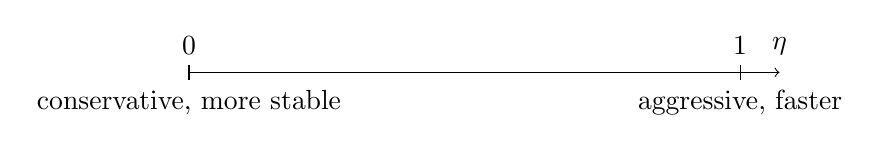
\begin{tikzpicture}
    \draw [->] (0,0) -- (7.5,0);
    \draw (0,0.1) -- + (0,0) node[above] {$0$};
    \draw (7,0.1) -- + (0,0) node[above] {$1$};
    \draw (7.5,0.1) -- + (0,0) node[above] {$\eta$};
    \draw (0,0.1) -- + (0,-0.2) node[below] {conservative, more stable};
    \draw (7,0.1) -- + (0,-0.2) node[below] {aggressive, faster};
\end{tikzpicture}
\end{figure}
% Strategies:
\begin{itemize}
    \item Constant: $\eta = 0.1$
    \item Decreasing, decaying: $\eta = 1/\sqrt{\text{\# updates made so far}}$
\end{itemize}
% 
A suggested form for the step size is to set the initial step size to $1$ and let the step size decrease as the inverse of the square root of the number of updates we've taken so far.
There are some nice theoretical results showing that SGD is guaranteed to converge in this case.\sidenote{provided all your gradients have bounded length}

\begin{algorithm}
\begin{juliaverbatim}
mutable struct Decay
    i # iteration
end

import Base.*
*(δη::Decay, x) = 1/sqrt(δη.i+=1) * x
\end{juliaverbatim}

\caption[][5mm]{
    \label{alg:step_size_decay}
    Inverse square root \textit{step size decay}. The iteration \jlv{i} will automatically increment every time the \jlv{Decay} is multiplied.
}
\end{algorithm}

% subsection step_size (end)

\subsection{Summary} % (fold)
\label{sub:summary}
% Done for linear regression; what about classification? % DIFF: Removed.
% 
In summary we have seen ($1$) the functions we're considering (linear predictors),
($2$) the criterion for choosing one (loss minimization),
and ($3$) an algorithm that goes after that criterion (SGD).
% 
We already worked out a linear regression example.
What are good loss functions for binary classification?
\begin{enumerate}
    \item \textbf{Linear predictors}:
    \[
        f_{\w}(x) \text{ based on score } \w\cdot\phi(x)
    \]

    \item \textbf{Loss minimization}: learning as optimization
    \[
        \minimize_{\w} \TrainLoss(\w)
    \]

    \item \textbf{Stochastic gradient descent}: optimization algorithm
    \[
        \w \leftarrow \w - \eta \nabla_{\w} \Loss(x,y,\w)
    \]
\end{enumerate}
% subsection summary (end)

% \pagebreak % TODO: MAYBE THIS ONE

\subsection{Zero-One Loss} % (fold)
\label{sub:zero_one_loss}
\begin{marginfigure}
  \caption{
    \label{fig:zero_one_loss_2} \textit{Zero-one loss}.
  }
  \begin{jlcode}
  p = let
      ymin = 0
      ymax = 4

      plots = Plots.Plot[
          Plots.Linear(
              x->Loss_01(x, +1, [1], x->x), (-3,3), xbins=1000, style="solid, ultra thick, mark=none, red", legendentry=L"\ZeroOneLoss"
          ),
      ]
      Axis(plots,
           xlabel=L"\text{margin}~(\mathbf{w}\cdot\phi(x))y",
           ylabel=L"\ZeroOneLoss(x,y,\mathbf{w})",
           style="ymajorgrids, enlarge x limits=0, ymin=$ymin, ymax=$ymax, legend pos=north west, legend style={at={(0.5,-0.5)},anchor=north}",
           width="5cm", height="4cm")
  end
  plot(p)
  \end{jlcode}
  \begin{center}
    \plot{fig/zero_one_loss_2}
  \end{center}
\end{marginfigure}
\begin{equation*}
    \ZeroOneLoss(x, y, \w) = \mathbb{1}[(\w \cdot \phi(x)) y \le 0]
\end{equation*}
Recall that we have the zero-one loss for classification.
But the main problem with zero-one loss is that it's hard to optimize (in fact, it's provably NP hard in the worst case).
And in particular, we cannot apply gradient-based optimization to it,
because the gradient is zero (almost) everywhere.
\begin{algorithm}
\begin{juliaverbatim}
Loss_01(x, y, 𝐰, φ) = 𝕀(margin(x, y, 𝐰, φ) ≤ 0)
\end{juliaverbatim}

% \caption{
%     \label{alg:zero_one_loss_2}
%     The \textit{zero-one loss} function, duplicate of \cref{alg:zero_one_loss} for convenience.
% }
\end{algorithm}
%

\noindent Problems with zero-one loss:
\begin{itemize}
    \item Gradient of $\ZeroOneLoss$ is $0$ everywhere, therefore SGD is not applicable.
    \item $\ZeroOneLoss$ is insensitive to how badly the model messed up.
\end{itemize}


% subsection zero_one_loss (end)    

\subsection{Hinge Loss (SVMs)} % (fold)
\label{sub:hinge_loss}
\[
    \HingeLoss(x, y, \w) = \max\{1 - (\w \cdot \phi(x)) y, 0 \}
\]
Hinge loss upper bounds $\ZeroOneLoss$ and has a non-trivial gradient. Try to increase the margin if it is less than $1$.
% 
To fix this problem, we can use the \textit{hinge loss}, which is an upper bound on the zero-one loss.
Minimizing upper bounds are a general idea; the hope is that pushing down the upper bound leads
to pushing down the actual function.
\begin{algorithm}
\begin{juliaverbatim}
Loss_hinge(x, y, 𝐰, φ) = max(1 - margin(x, y, 𝐰, φ), 0)
\end{juliaverbatim}
\caption[][-10mm]{
    \label{alg:hinge_loss}
    The \textit{hinge loss} function, an upper bound on the \textit{zero-one} loss function.
}
\end{algorithm}

Advanced: The hinge loss corresponds to the \textit{Support Vector Machine} (SVM) objective function with one important difference.
The SVM objective function also includes a \textit{regularization penalty} $\|\w\|^2$, which prevents the weights from getting too large.
We will get to regularization later in the course, so you needn't worry about this for now.
But if you're curious, read on.
\begin{marginfigure}
  \begin{jlcode}
    p = let
        ymin = 0
        ymax = 4

        plots = Plots.Plot[
            Plots.Linear(
                x->Loss_01(x, +1, [1], x->x), (-3,3), xbins=1000, style="solid, ultra thick, mark=none, red", legendentry=L"\ZeroOneLoss"
            ),
            Plots.Linear(
                x->Loss_hinge(x, +1, [1], x->x), (-3,3), style="solid, ultra thick, mark=none, darkgreen", legendentry=L"\HingeLoss"
            ),
        ]
        Axis(plots,
             xlabel=L"\text{margin}~(\mathbf{w}\cdot\phi(x))y",
             ylabel=L"\Loss(x,y,\mathbf{w})",
             style="ymajorgrids, enlarge x limits=0, ymin=$ymin, ymax=$ymax, legend pos=north west, legend style={at={(0.5,-0.5)},anchor=north}",
             width="5cm", height="4cm")
    end
    plot(p)
  \end{jlcode}
  \begin{center}
    \plot{fig/hinge_loss}
  \end{center}
  \caption{
    \label{fig:hinge_loss} \textit{Hinge loss}.
  }
\end{marginfigure}

Why should we penalize $\|\w\|^2$?  One answer is Occam's razor, which says to find the simplest hypothesis that explains the data.
Here, simplicity is measured in the length of $\w$.  This can be made formal using statistical learning theory (take CS229T if you want to learn more).

Perhaps a less abstract and more geometric reason is the following.
Recall that we defined the (algebraic) margin to be $\w \cdot \phi(x) y$.
The actual (signed) distance from a point to the decision boundary
is actually $\frac{\w}{\|\w\|} \cdot \phi(x) y$, this is called the geometric margin.
So the loss being zero (that is, $\HingeLoss(x,y,\w) = 0$) is equivalent to
the algebraic margin being at least $1$ (that is, $\w \cdot \phi(x) y \ge 1$),
which is equivalent to the geometric margin being larger than $\frac1{\|\w\|}$ (that is, $\frac{\w}{\|\w\|} \cdot \phi(x) y \ge \frac1{\|\w\|}$).
Therefore, reducing $\|\w\|$ increases the geometric margin.
For this reason, SVMs are also referred to as \textit{max-margin} classifiers.
\begin{algorithm}
\begin{juliaverbatim}
geometric_margin(x, y, 𝐰, φ) = 𝐰/norm(𝐰)⋅φ(x)*y
\end{juliaverbatim}

\caption{
    \label{alg:geometric_margin}
    The \textit{geometric margin} is the signed distance from a point to a decision boundary.
}
\end{algorithm}
% subsection hinge_loss_ (end)

\subsection{Logistic Regression} % (fold)
\label{sub:logistic_regression}
\[
    \LogisticLoss(x, y, \w) = \log(1 + e^{-(\w \cdot \phi(x)) y})
\]
% \textbf{Intuition:}
Try to increase margin even when it already exceeds $1$.
% 
Another popular loss function used in machine learning is the \textit{logistic loss}.
\begin{algorithm}
\begin{juliaverbatim}
Loss_logistic(x, y, 𝐰, φ) = log(1 + exp(-margin(x, y, 𝐰, φ)))
\end{juliaverbatim}

\caption{
    \label{alg:logistic_locc}
    The \textit{logistic loss} function.
}
\end{algorithm}

The main property of the logistic loss is no matter how correct your prediction is, you will have non-zero loss,
and so there is still an incentive (although a diminishing one) to push the margin even larger.
This means that you'll update on every single example.
There are some connections between logistic regression and probabilistic models, which we will get to later.
\begin{marginfigure}
  \begin{jlcode}
    p = let
        ymin = 0
        ymax = 4

        plots = Plots.Plot[
            Plots.Linear(
                x->Loss_01(x, +1, [1], x->x), (-3,3), xbins=1000, style="solid, ultra thick, mark=none, red", legendentry=L"\ZeroOneLoss"
            ),
            Plots.Linear(
                x->Loss_hinge(x, +1, [1], x->x), (-3,3), style="solid, ultra thick, mark=none, darkgreen", legendentry=L"\HingeLoss"
            ),
            Plots.Linear(
                x->Loss_logistic(x, +1, [1], x->x), (-3,3), style="solid, ultra thick, mark=none, sun", legendentry=L"\LogisticLoss"
            ),
        ]
        Axis(plots,
             xlabel=L"\text{margin}~(\mathbf{w}\cdot\phi(x))y",
             ylabel=L"\Loss(x,y,\mathbf{w})",
             style="ymajorgrids, enlarge x limits=0, ymin=$ymin, ymax=$ymax, legend pos=north west, legend style={at={(0.5,-0.5)},anchor=north}",
             width="5cm", height="4cm")
    end
    plot(p)
  \end{jlcode}
  \begin{center}
    \plot{fig/logistic_loss}
  \end{center}
  \caption{
    \label{fig:logistic_loss} \textit{Logistic loss}.
  }
\end{marginfigure}
% section logistic_regression (end)

\pagebreak

\begin{overflowexample}
    \bparagraph{A gradient exercise.} Compute the gradient of the hinge loss:
    \[
        \HingeLoss(x, y, \w) = \max\{1 - (\w \cdot \phi(x)) y, 0 \}
    \]
    You should try to ``see'' the solution before you write things down formally.
    Pictorially, it should be evident: when the margin is less than $1$,
    then the gradient is the gradient of $1-(\w\cdot\phi(x))y$, which is equal to $-\phi(x) y$.
    If the margin is larger than $1$, then the gradient is the gradient of $0$, which is $0$.
    % Combining the two cases: % DIFF
    \[
        \displaystyle \nabla_{\w} \HingeLoss(x, y, \w) =
        \begin{cases}
        -\phi(x) y & \text{if $\w\cdot\phi(x) y < 1$} \\
        0 & \text{if $\w\cdot\phi(x) y > 1$}
        \end{cases}
    \]
    What about when the margin is exactly $1$?
    Technically, the gradient doesn't exist because the hinge loss is not differentiable there.
    %#% DIFF: removed:
    % Fear not! 
    % , at the end of the day
    Practically speaking, we can take either $-\phi(x) y$ or $0$ (or anything in between).
\br\\
\begin{exalgorithm}
\begin{juliaverbatim}
∇Loss_hinge(x, y, 𝐰, φ) = margin(x, y, 𝐰, φ) < 1 ? -φ(x)*y : 0
\end{juliaverbatim}
\end{exalgorithm}

    Technical note (can be skipped): given $f(\w)$, the gradient $\nabla f(\w)$ is only defined at points $\w$ where $f$ is differentiable.
    However, subdifferentials $\partial f(\w)$ are defined at every point (for convex functions).
    The subdifferential is a set of vectors called subgradients $z \in f(\w)$ which define linear underapproximations to $f$,
    namely $f(\w) + z \cdot (\w^\prime - \w) \le f(\w^\prime)$ for all $\w^\prime$.
\end{overflowexample}

% \begin{equation*}
%     \underbrace{\w \cdot \phi(x)}_{\text{score}}
% \end{equation*}
\subsection{Summary} % (fold)
\label{sub:summary}
\begin{table}[!h]
  \centering
  \caption{
    \label{tab:ml1} Summary of machine learning.
  }
  % $\underbrace{\w \cdot \phi(x)}_{\text{score}}$
  \begin{tabular}{lll}
    \toprule
    $\text{score} = \w \cdot \phi(x)$ & \textbf{Classification} & \textbf{Regression} \\
    \midrule
    \textbf{Predictor} $f_{\w}$ & $\sign(\text{score})$ & $\text{score}$\\
    \\
    \textbf{Relate to correct} $y$ & margin $(\text{score}\cdot y)$ & residual $(\text{score} - y)$\\
    \\
    \shortstack[l]{\textbf{Loss functions}\\\phantom{---}\\\phantom{---}} & \shortstack[l]{\text{zero-one}\\\text{hinge}\\\text{logistic}} & \shortstack[l]{squared\\absolute deviation}\\
    \\
    \textbf{Algorithm} & stochastic gradient descent & stochastic gradient descent\\
    \bottomrule
  \end{tabular}
\end{table}

% TODO: "Next lecture/chapter" side note.

% subsection summary (end)

% chapter machine_learning_i (end)